% Name: Hash table with chaining
% Description: Five buckets indexed by the key's hash, with the keys that hash to the same bucket chained in a list.
% Tags: hash table, hashing, collisions, chaining

\usetikzlibrary{arrows.meta, positioning}

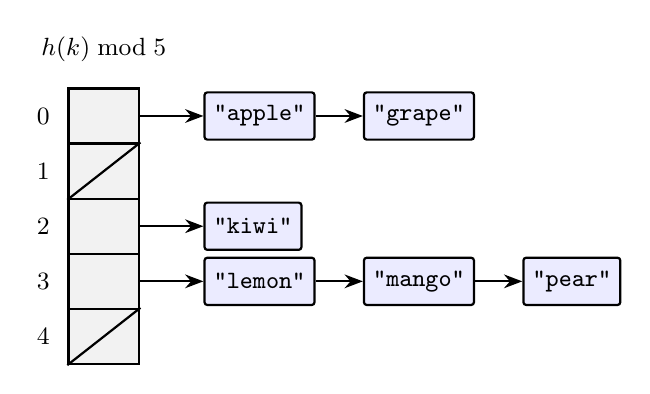
\begin{tikzpicture}[>={Stealth}, bucket/.style={draw, thick, minimum width=9mm, minimum height=7mm, fill=gray!10},
    entry/.style={draw, thick, rounded corners=1pt, minimum height=6mm, fill=blue!8, font=\ttfamily\small}]
  \foreach \i in {0,...,4} {
    \node[bucket] (b\i) at (0,-\i*0.7) {};
    \node[left=1mm of b\i, font=\small] {\i};
  }
  \node[entry, right=8mm of b0] (e1) {"apple"};
  \node[entry, right=6mm of e1] (e2) {"grape"};
  \node[entry, right=8mm of b2] (e3) {"kiwi"};
  \node[entry, right=8mm of b3] (e4) {"lemon"};
  \node[entry, right=6mm of e4] (e5) {"mango"};
  \node[entry, right=6mm of e5] (e6) {"pear"};
  \foreach \a/\b in {b0/e1, e1/e2, b2/e3, b3/e4, e4/e5, e5/e6} \draw[->, thick] (\a) -- (\b);
  \foreach \i in {1,4} \draw[thick] (b\i.south west) -- (b\i.north east);
  \node[above=2mm of b0, font=\small] {$h(k) \bmod 5$};
\end{tikzpicture}
